\documentclass[article]{jss}

%% -- LaTeX packages and custom commands ---------------------------------------

%% recommended packages
\usepackage{thumbpdf,lmodern}
\usepackage{amsmath}

%% another package (only for this demo article)
\usepackage{framed}

%% new custom commands
\newcommand{\class}[1]{`\code{#1}'}
\newcommand{\fct}[1]{\code{#1()}}

%% For Sweave-based articles about R packages:
%% need no \usepackage{Sweave}



%% -- Article metainformation (author, title, ...) -----------------------------

%% - \author{} with primary affiliation (and optionally ORCID link)
%% - \Plainauthor{} without affiliations
%% - Separate authors by \And or \AND (in \author) or by comma (in \Plainauthor).
%% - \AND starts a new line, \And does not.
\author{Dan MacLean\\The Sainsbury Laboratory}
\Plainauthor{Dan MacLean}

%% - \title{} in title case
%% - \Plaintitle{} without LaTeX markup (if any)
%% - \Shorttitle{} with LaTeX markup (if any), used as running title
\title{\pkg{peppwR}: Simulation-Based Power Analysis for Phosphoproteomics Experiments in \proglang{R}}
\Plaintitle{peppwR: Simulation-Based Power Analysis for Phosphoproteomics Experiments in R}
\Shorttitle{\pkg{peppwR}: Power Analysis for Phosphoproteomics}

%% - \Abstract{} almost as usual
\Abstract{
Phosphoproteomics experiments require careful experimental design to ensure
adequate statistical power, yet no dedicated tools exist for power analysis
that account for the unique statistical properties of peptide-level
quantification data. We present \pkg{peppwR}, an \proglang{R} package for
simulation-based power analysis tailored to phosphoproteomics. \pkg{peppwR}
fits distributions to pilot data on a per-peptide basis, capturing the
heterogeneity in abundance and variance across the peptidome. It supports
multiple statistical tests (Wilcoxon, bootstrap-$t$, Bayes factor), tracks
missingness patterns common in mass spectrometry data, and provides
FDR-aware power calculations. Users can determine required sample sizes,
estimate power for planned experiments, or identify minimum detectable effect sizes.
}

%% - \Keywords{} with LaTeX markup, at least one required
%% - \Plainkeywords{} without LaTeX markup (if necessary)
%% - Should be comma-separated and in sentence case.
\Keywords{power analysis, phosphoproteomics, mass spectrometry, experimental design, \proglang{R}}
\Plainkeywords{power analysis, phosphoproteomics, mass spectrometry, experimental design, R}

%% - \Address{} of at least one author
%% - May contain multiple affiliations for each author
%%   (in extra lines, separated by \emph{and}\\).
%% - May contain multiple authors for the same affiliation
%%   (in the same first line, separated by comma).
\Address{
  Dan MacLean\\
  The Sainsbury Laboratory\\
  University of East Anglia\\
  Norwich NR4 7UH, UK\\
  E-mail: \email{dan.maclean@tsl.ac.uk}\\
  URL: \url{https://github.com/TeamMacLean/peppwR}
}

\begin{document}

\section{Introduction} \label{sec:intro}

% Statistical Power Foundation
Statistical power---the probability of correctly rejecting a false null hypothesis---represents one of the most fundamental concepts in experimental design \citep{cohen1988power}. Introduced by \citet{neyman1933} and formalized by \citet{cohen1962}, power analysis provides the theoretical framework for determining appropriate sample sizes, estimating the likelihood of detecting true effects, and identifying minimum detectable effect sizes. The consequences of inadequate power are profound: under-powered studies waste resources and risk missing genuine biological discoveries.

Despite some adoption in clinical trials \citep{schulz2005sample}, power analysis remains systematically neglected in proteomics research. Most published proteomics studies do not report formal power calculations, in contrast to higher reporting rates observed in clinical research domains. This disparity persists despite the field's evolution toward increasingly quantitative approaches and the availability of sophisticated statistical methods for proteomics data analysis \citep{karp2010addressing}.

% Proteomics-Specific Challenges
Mass spectrometry-based proteomics presents unique statistical challenges that violate fundamental assumptions of traditional power analysis. Peptide abundances exhibit extreme heterogeneity, with concentrations spanning multiple orders of magnitude within a single experiment \citep{olsen2006phosphoproteomics, humphrey2015phosphoproteomics}. This heterogeneity extends beyond mean abundances to encompass dramatic differences in variance structure across the peptidome \citep{karp2010addressing}. Abundance distributions can deviate substantially from normality, typically exhibiting right skewness that may be better characterized by alternative distributions such as gamma, lognormal, or inverse Gaussian models \citep{webb2015mnar}. These distributional properties reflect both biological variation and the multiplicative nature of mass spectrometry quantification processes.

Missing values in proteomics follow systematic, non-random patterns that fundamentally alter statistical inference. Low-abundance peptides are disproportionately affected by detection limits, creating missing-not-at-random (MNAR) data structures \citep{webb2015mnar, lazar2016mnar}. The proportion of missing values can exceed 50\% in discovery proteomics experiments \citep{tyanova2016imputation}, with missingness rates negatively correlated with abundance levels---a pattern that violates the missing-completely-at-random (MCAR) assumptions underlying most statistical tests. Fourth, phosphoproteomics experiments routinely quantify thousands of peptides simultaneously, necessitating multiple testing corrections that substantially reduce effective statistical power \citep{karp2010addressing, zhang2018multiple}.

% Existing Tool Analysis
Current power analysis tools address these proteomics-specific challenges incompletely or not at all (Table~\ref{tab:tool-comparison}). \pkg{Perseus} \citep{tyanova2016perseus}, a widely-used analysis platform in proteomics, provides comprehensive statistical analysis including t-tests, ANOVA, and volcano plots, but offers no power analysis functionality. Users must rely on generic tools or ad-hoc approaches for experimental design decisions. \pkg{MSstats} \citep{chang2012msstats} provides sophisticated variance component modeling through linear mixed models and supports analysis at both peptide and protein levels, but utilizes aggregate variance components from fitted models rather than individual per-peptide distribution modeling needed for comprehensive phosphoproteomics experimental design. The \pkg{clippda} package \citep{nyangoma2012clippda} was specifically designed for SELDI-TOF peak data and incorporates routines for handling data heterogeneities, but remains primarily focused on older mass spectrometry platforms rather than modern LC-MS/MS phosphoproteomics applications. \pkg{G*Power} \citep{gpower}, while widely used across scientific disciplines with over 30,000 citations, assumes normality and homogeneous variance, making it inappropriate for proteomics applications where data violate these assumptions. \pkg{MultiPower} \citep{tarazona2020multipower} addresses power analysis in multi-omics contexts and is designed for integrative analysis across multiple platforms (genomics, transcriptomics, metabolomics), with limited focus on the specific statistical challenges of proteomics-only experiments. The tool focuses on pathway-level analysis rather than individual protein or peptide quantification.

The absence of tools that combine per-peptide distribution modeling with realistic missing data patterns and FDR-aware calculations has led researchers to either skip power analysis entirely or apply inappropriate methods, potentially contributing to reproducibility issues and missed conclusions. This methodological gap is particularly problematic given the high costs associated with proteomics experiments and the limited sample availability in many contexts.

% peppwR Positioning
\pkg{peppwR} is an \proglang{R} package that directly addresses these limitations through simulation-based power analysis tailored specifically to mass spectrometry proteomics data. \pkg{peppwR} implements per-peptide distribution fitting to capture abundance heterogeneity, supports multiple statistical tests appropriate for non-normal data, incorporates realistic missing data patterns, and provides FDR-aware power calculations for high-throughput experiments. The package operates in two complementary modes: aggregate analysis for preliminary design decisions without pilot data, and per-peptide analysis that leverages pilot data to provide detailed, peptide-specific power estimates.

\pkg{peppwR} answers the three fundamental experimental design questions: ``What sample size do I need to achieve target power?'', ``What statistical power will my planned experiment achieve?'', and ``What is the minimum detectable effect size given my sample size constraints?'' By addressing the unique statistical properties of proteomics data, \pkg{peppwR} enables more informed experimental design decisions and contributes to improving the reproducibility and efficiency of proteomics research.

\begin{table}[ht]
\centering
\caption{Comparison of power analysis tools for proteomics applications.}
\label{tab:tool-comparison}
\begin{tabular}{lcccccc}
\hline
Tool & \begin{tabular}[c]{@{}c@{}}Proteomics\\Focus\end{tabular} & \begin{tabular}[c]{@{}c@{}}Per-feature\\Modeling\end{tabular} & \begin{tabular}[c]{@{}c@{}}Non-normal\\Distributions\end{tabular} & \begin{tabular}[c]{@{}c@{}}Missing Data\\Handling\end{tabular} & \begin{tabular}[c]{@{}c@{}}Multiple\\Testing\end{tabular} & \begin{tabular}[c]{@{}c@{}}Statistical\\Tests\end{tabular} \\
\hline
\pkg{peppwR} & x & x & x & x & x & \begin{tabular}[c]{@{}c@{}}Wilcoxon, Bootstrap-$t$\\Bayes Factor\end{tabular} \\
\pkg{MSstats} & x & --\footnote{Aggregate variance components} & x & x & x & Linear mixed models \\
\pkg{Perseus} & x & -- & x & x & x & \begin{tabular}[c]{@{}c@{}}t-test, ANOVA\\Volcano plots\end{tabular} \\
\pkg{clippda} & --\footnote{SELDI-TOF specific} & -- & -- & -- & -- & t-test \\
\pkg{MultiPower} & --\footnote{Multi-omics integration} & x & -- & -- & x & Various \\
\pkg{G*Power} & -- & -- & -- & -- & -- & \begin{tabular}[c]{@{}c@{}}t-test, ANOVA\\Correlation\end{tabular} \\
\hline
\end{tabular}
\end{table}

%% -- Methods and Implementation -----------------------------------------------

\section{Methods and Implementation} \label{sec:methods}

\pkg{peppwR} implements simulation-based power analysis through a modular framework that addresses the unique statistical challenges of phosphoproteomics data. The package operates in two complementary modes: aggregate analysis for preliminary design decisions without pilot data, and per-peptide analysis that leverages pilot data to provide detailed, peptide-specific power estimates across the heterogeneous peptidome.


\subsection{Statistical Framework}

Statistical power, defined as $P(reject H_0 | H_1 \text{ true}) = 1 - \beta$ (where $\beta$ is the Type II error rate), provides the theoretical foundation for experimental design decisions. For a given statistical test with significance level $\alpha$, power depends on the effect size $\delta$, sample size $n$, and the underlying population distributions. In the context of proteomics experiments comparing two groups, we test the null hypothesis $H_0: \mu_{\text{treatment}} = \mu_{\text{control}}$ against the alternative $H_1: \mu_{\text{treatment}} \neq \mu_{\text{control}}$.

\pkg{peppwR} accommodates three fundamental experimental design questions through constrained optimization. When \code{find = "sample\_size"}, the package determines the minimum $n$ required to achieve target power $\pi_{\text{target}}$:
\begin{equation}
n^* = \min\{n : P(reject H_0 | \delta, n) \geq \pi_{\text{target}}\}
\end{equation}

When \code{find = "power"}, it estimates the expected power for a fixed sample size:
\begin{equation}
\pi(n, \delta) = P(reject H_0 | \delta, n)
\end{equation}

When \code{find = "effect\_size"}, it identifies the minimum detectable effect size:
\begin{equation}
\delta^* = \min\{\delta : P(reject H_0 | \delta, n) \geq \pi_{\text{target}}\}
\end{equation}

The effect size is parameterized as a multiplicative factor $\delta$ such that treatment group abundances are scaled by $\delta$ relative to control abundances. This multiplicative parameterization naturally accommodates the log-scale nature of mass spectrometry quantification, where biological effects typically manifest as fold-changes rather than additive differences.

In per-peptide mode, power calculations are performed independently for each peptide $i$ with fitted distribution parameters $\theta_i$, yielding peptide-specific power estimates $\pi_i(n, \delta)$. The package then reports the proportion of peptides achieving target power:
\begin{equation}
P_{\text{peptidome}}(n, \delta, \pi_{\text{target}}) = \frac{1}{K}\sum_{i=1}^{K} \mathbf{1}[\pi_i(n, \delta) \geq \pi_{\text{target}}]
\end{equation}
where $K$ is the total number of peptides and $\mathbf{1}[\cdot]$ is the indicator function.

For FDR-aware analysis, power is evaluated after Benjamini-Hochberg correction. Let $p_{(1)} \leq p_{(2)} \leq \ldots \leq p_{(m)}$ denote the ordered p-values from $m$ tests. The FDR-controlling procedure rejects all hypotheses $H_{(i)}$ for $i \leq k^*$, where:
\begin{equation}
k^* = \max\left\{i : p_{(i)} \leq \frac{i \cdot \alpha}{m}\right\}
\end{equation}

Power under FDR correction becomes the expected proportion of true positives among discoveries, accounting for the adaptive threshold imposed by the multiple testing procedure.

\subsection{Distribution Fitting}

\pkg{peppwR} models peptide abundance distributions using maximum likelihood estimation across multiple parametric families. The core distributions supported are gamma ($\text{Gamma}(\alpha, \beta)$), lognormal ($\text{LogNormal}(\mu, \sigma^2)$), normal ($\text{Normal}(\mu, \sigma^2)$), and inverse Gaussian ($\text{InverseGaussian}(\mu, \lambda)$). These distributions capture the right-skewed, positive-valued nature of mass spectrometry intensities while accommodating varying degrees of skewness and heteroscedasticity observed across the peptidome.

For each peptide $i$ with observed abundances $\mathbf{x}_i = \{x_{i1}, x_{i2}, \ldots, x_{in_i}\}$, the package fits each candidate distribution with probability density function $f_k(x | \theta_k)$ by maximizing the log-likelihood:
\begin{equation}
\hat{\theta}_{k,i} = \arg\max_{\theta_k} \sum_{j=1}^{n_i} \log f_k(x_{ij} | \theta_k)
\end{equation}

Model selection employs the Akaike Information Criterion (AIC), selecting the distribution with minimum AIC score:
\begin{equation}
\hat{k}_i = \arg\min_k \left\{-2 \sum_{j=1}^{n_i} \log f_k(x_{ij} | \hat{\theta}_{k,i}) + 2p_k\right\}
\end{equation}
where $p_k$ is the number of parameters in distribution $k$.

The gamma distribution, parameterized by shape $\alpha > 0$ and rate $\beta > 0$, provides flexibility in modeling right-skewed abundance data with controlled variance-to-mean relationships. The lognormal distribution naturally accommodates multiplicative biological processes underlying protein expression, while the inverse Gaussian distribution offers an intermediate option between gamma and lognormal with distinct tail behavior. Additional candidate distributions including Weibull, exponential, and beta (for transformed data) are available through the \pkg{univariateML} interface.

Parameter estimation leverages the \pkg{fitdistrplus} package for standard distributions and \pkg{univariateML} for specialized cases. Both packages implement numerically stable algorithms with appropriate handling of boundary conditions and convergence diagnostics. When maximum likelihood estimation fails due to insufficient data, extreme parameter estimates, or numerical instability, \pkg{peppwR} provides three fallback strategies controlled by the \code{on\_fit\_failure} argument.

The \code{"exclude"} strategy removes problematic peptides from analysis, reporting the exclusion count for transparency. The \code{"empirical"} strategy substitutes parametric distributions with empirical bootstrap resampling from observed values, preserving the exact empirical distribution at the cost of reduced statistical efficiency. The \code{"lognormal"} strategy fits a moment-matched lognormal distribution using method-of-moments estimates, providing a robust fallback when maximum likelihood fails but ensuring all peptides remain in analysis.

Distribution fitting diagnostics include goodness-of-fit statistics (Kolmogorov-Smirnov, Anderson-Darling), QQ plots comparing theoretical and empirical quantiles, and density overlay plots visualizing the fitted distribution against observed data histograms. These diagnostics enable users to assess the adequacy of distributional assumptions and identify peptides where parametric modeling may be inappropriate.

\subsection{Simulation Engine}

Power estimation employs Monte Carlo simulation to accommodate the complex statistical properties of proteomics data that preclude analytical power calculations. The simulation framework generates synthetic datasets under specified experimental conditions, applies statistical tests, and estimates power as the proportion of simulations achieving statistical significance.

For each peptide $i$ with fitted distribution $f_i(\cdot | \hat{\theta}_i)$ and each candidate sample size $n$, the simulation algorithm proceeds as follows:

\begin{enumerate}
\item Generate $n$ control group samples: $X_{i,\text{control}}^{(s)} \sim f_i(\cdot | \hat{\theta}_i)$ for $s = 1, \ldots, n$
\item Generate $n$ treatment group samples: $X_{i,\text{treatment}}^{(s)} \sim f_i(\cdot | \delta \cdot \hat{\theta}_i)$ for $s = 1, \ldots, n$, where $\delta$ represents the multiplicative effect size
\item Apply missing data patterns if \code{include\_missingness = TRUE}, randomly removing observations according to the peptide-specific missingness rate $r_i$
\item Compute the test statistic and p-value using the specified statistical test
\item Record rejection outcome: $R^{(j)} = \mathbf{1}[p^{(j)} \leq \alpha]$ for simulation $j$
\item Repeat for $n_{\text{sim}}$ independent simulations
\end{enumerate}

Power is estimated as:
\begin{equation}
\hat{\pi}_i(n, \delta) = \frac{1}{n_{\text{sim}}} \sum_{j=1}^{n_{\text{sim}}} R^{(j)}
\end{equation}

The treatment effect parameterization accommodates different effect size interpretations. For location-scale families, the effect size $\delta$ scales the location parameter (mean for normal, rate parameter for gamma, location parameter for lognormal). This multiplicative scaling preserves the distributional shape while shifting the central tendency, consistent with biological interpretation of fold-changes in proteomics.

The default $n_{\text{sim}} = 1000$ simulations provides adequate precision for most applications, but can be increased for higher precision requirements.

The simulation engine supports vectorized operations across peptides and sample sizes, enabling efficient computation of power curves and sample size determinations. Parallel processing capabilities allow distribution across multiple CPU cores when analyzing large peptidomes, with linear scaling up to the number of available cores.

For FDR-aware simulations, the engine generates complete experiments across all peptides simultaneously, applies the Benjamini-Hochberg procedure to the resulting p-value vectors, and computes power as the proportion of true positives among discoveries. This approach correctly accounts for the dependence structure introduced by multiple testing correction, providing realistic power estimates for high-throughput experiments.

\subsection{Missing Data Handling}

\pkg{peppwR} incorporates missing data mechanisms specific to mass spectrometry-based proteomics, where detection limits create systematic patterns of missing-not-at-random (MNAR) data. The package implements a two-level approach to characterizing and incorporating missingness patterns into power calculations.

At the dataset level, \pkg{peppwR} detects MNAR patterns by computing the Spearman correlation between peptide-level mean abundances and missingness rates. A significant negative correlation ($\rho < -0.3$, $p < 0.05$) indicates that low-abundance peptides are systematically more likely to be missing---the signature of detection-limit-driven MNAR common in discovery proteomics \citep{webb2015mnar}. This dataset-level diagnostic provides users with quantitative evidence for MNAR mechanisms and informs the interpretation of power analysis results.

The MNAR detection algorithm computes peptide-specific summary statistics:
\begin{align}
\bar{x}_i &= \frac{1}{n_{\text{obs},i}} \sum_{j: x_{ij} \neq \text{NA}} x_{ij} \\
r_i &= \frac{n_{\text{missing},i}}{n_{\text{total},i}}
\end{align}
where $\bar{x}_i$ is the mean abundance for peptide $i$ (excluding missing values), $r_i$ is the missingness rate, $n_{\text{obs},i}$ is the number of observed values, and $n_{\text{missing},i}$ is the number of missing values.

At the peptide level, the package records the observed missingness rate $r_i$ for each peptide during the distribution fitting phase. When \code{include\_missingness = TRUE} is specified in power analysis, simulations incorporate these peptide-specific NA rates by randomly removing observations from generated samples with probability $r_i$. This approach preserves the heterogeneous pattern of data loss across peptides while maintaining the stochastic nature of missing data generation.

The missing data incorporation algorithm modifies the standard simulation procedure:
\begin{enumerate}
\item Generate complete control and treatment samples as described above
\item For each peptide $i$, randomly select $\lfloor n \cdot r_i \rfloor$ observations for removal from each group
\item Apply the specified statistical test to the resulting incomplete data
\item Record the test outcome, including cases where insufficient data remains for testing
\end{enumerate}

When missingness results in insufficient data for statistical testing (typically when fewer than 3 observations remain in either group), the peptide is excluded from that simulation iteration. The proportion of successful tests is reported alongside power estimates, providing transparency about the impact of missing data on statistical inference.

This missingness-aware simulation provides realistic power estimates that account for expected data loss, enabling more accurate sample size determinations for experiments anticipated to have substantial missing values. Users can compare power estimates with and without missingness incorporation to quantify the impact of incomplete data on experimental design requirements.

\subsection{Software Architecture}

\pkg{peppwR} implements an S3 object-oriented architecture with two primary classes: \class{peppwr\_fits} and \class{peppwr\_power}, each equipped with specialized methods for printing, plotting, and summarization.

The \class{peppwr\_fits} class encapsulates distribution fitting results, storing fitted parameters, goodness-of-fit statistics, and metadata for each peptide. The class structure includes:
\begin{itemize}
\item \code{data}: Original input data as nested tibble
\item \code{fits}: List of fit result tibbles per peptide containing distribution names, log-likelihood values, and AIC scores
\item \code{best}: Character vector indicating the best-fitting distribution for each peptide
\item \code{call}: Original function call for reproducibility
\item \code{missingness}: Tibble with peptide-level missingness rates and diagnostic statistics (optional)
\item \code{dataset\_mnar}: Dataset-level MNAR correlation metric and interpretation (optional)
\end{itemize}

The \class{peppwr\_power} class stores power analysis results with associated simulation parameters:
\begin{itemize}
\item \code{mode}: Analysis mode ("aggregate" or "per\_peptide")
\item \code{question}: The solved question ("power", "sample\_size", or "effect\_size")
\item \code{answer}: The computed result value
\item \code{simulations}: List containing simulation results and configuration details
\item \code{params}: List of input parameters used in the analysis
\item \code{call}: Original function call for reproducibility
\end{itemize}

Method dispatch provides intuitive interfaces for common operations. The \code{print()} methods deliver concise summaries appropriate for interactive analysis, while \code{summary()} methods provide detailed statistical output including confidence intervals and fit diagnostics. The \code{plot()} methods generate diagnostic visualizations tailored to each class.

The design separates core functionality into distinct components: distribution fitting (\fct{fit\_distributions}), power analysis (\fct{power\_analysis}), simulation engine (\fct{run\_power\_sim}), statistical tests (\fct{test\_wilcoxon}, \fct{test\_bootstrap\_t}, \fct{test\_bayes\_t}), and visualization (\fct{plot.peppwr\_fits}, \fct{plot.peppwr\_power}). This modular architecture enables flexible extension while maintaining clear separation of concerns.

%% -- Examples -----------------------------------------------------------------

\section{Examples} \label{sec:examples}
%% 3.1 Aggregate Mode Analysis
\subsection{Aggregate Mode Analysis}

The \pkg{peppwR} package implements two complementary analysis modes. Aggregate mode operates with user-specified distribution parameters rather than pilot data, providing rapid power estimates for experimental planning scenarios where pilot data is unavailable. This mode addresses the three fundamental power analysis questions through Monte Carlo simulation using parametric distributions.

\subsubsection{Distribution Parameterization}

Aggregate mode requires specification of a distribution family and associated parameters. The package accepts parameters as named lists corresponding to standard \proglang{R} distribution parameterizations.

\begin{Schunk}
\begin{Sinput}
R> library(peppwR)
\end{Sinput}
\end{Schunk}

For demonstration purposes, we use gamma distribution parameters with shape values ranging from 1.5 to 5 and rate parameters from 0.01 to 0.1. Lower shape parameters generate more skewed distributions with higher variance, while higher shape parameters produce more symmetric distributions with reduced variance.

\subsubsection{Sample Size Determination}

The \fct{power\_analysis} function determines required sample sizes through iterative simulation. When \code{find = "sample_size"}, the function identifies the minimum per-group sample size necessary to achieve a specified target power for a given effect size.

\begin{Schunk}
\begin{Sinput}
R> set.seed(123)
R> result <- power_analysis(
+    distribution = "gamma",
+    params = list(shape = 2, rate = 0.05),
+    effect_size = 2,
+    target_power = 0.8,
+    find = "sample_size",
+    n_sim = 1000
+  )
R> print(result)
\end{Sinput}
\begin{Soutput}
peppwr_power analysis
---------------------
Mode: aggregate

Recommended sample size: N=25 per group
Target power: 80%
Effect size: 2.00-fold

Statistical test: wilcoxon
Significance level: 0.05
\end{Soutput}
\end{Schunk}

The algorithm performs 1000 Monte Carlo simulations to identify the minimum sample size achieving the target power of 80\%, determining that 25 samples per group are required (Figure~\ref{fig:aggregate-power-curve}).

\begin{Schunk}
\begin{Sinput}
R> plot(result)
\end{Sinput}
\end{Schunk}

\begin{figure}[ht]
\centering
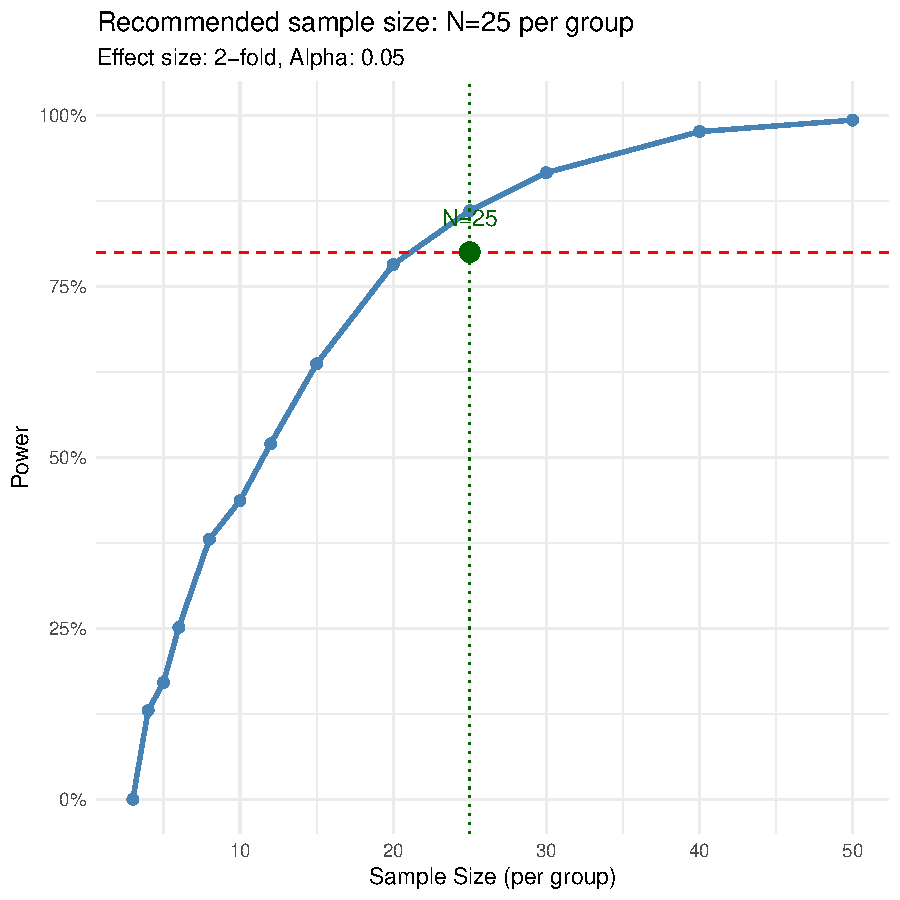
\includegraphics[width=0.7\textwidth]{jss-article-sample-size-plot}
\caption{Power curve showing the relationship between sample size and achieved power. The recommended sample size corresponds to the first value achieving the target power of 0.8.}
\label{fig:aggregate-power-curve}
\end{figure}

Figure~\ref{fig:aggregate-power-curve} demonstrates how statistical power increases with sample size, with the recommended value marked at the intersection with the target power threshold.

\subsubsection{Power Estimation}

Power estimation for fixed experimental designs operates through the \code{find = "power"} specification. This mode simulates experiments with predetermined sample sizes and effect sizes to estimate the probability of correctly rejecting false null hypotheses.

\begin{Schunk}
\begin{Sinput}
R> set.seed(123)
R> result <- power_analysis(
+    distribution = "gamma",
+    params = list(shape = 2, rate = 0.05),
+    effect_size = 2,
+    n_per_group = 6,
+    find = "power",
+    n_sim = 1000
+  )
R> print(result)
\end{Sinput}
\begin{Soutput}
peppwr_power analysis
---------------------
Mode: aggregate

Power: 24%
Sample size: 6 per group
Effect size: 2.00-fold

Statistical test: wilcoxon
Significance level: 0.05
\end{Soutput}
\end{Schunk}

The simulation reveals that 6 samples per group provide 24\% power to detect a 2-fold effect under the specified distributional assumptions, substantially below the conventional 80\% power threshold.

\subsubsection{Minimum Detectable Effect Size}

The package determines minimum detectable effect sizes through \code{find = "effect_size"} specifications. This analysis identifies the smallest multiplicative effect that can be reliably detected given sample size and power constraints (Figure~\ref{fig:aggregate-effect-curve}).

\begin{Schunk}
\begin{Sinput}
R> set.seed(123)
R> result <- power_analysis(
+    distribution = "gamma",
+    params = list(shape = 2, rate = 0.05),
+    n_per_group = 6,
+    target_power = 0.8,
+    find = "effect_size",
+    n_sim = 1000
+  )
R> print(result)
\end{Sinput}
\begin{Soutput}
peppwr_power analysis
---------------------
Mode: aggregate

Minimum detectable effect: 5.00-fold
Sample size: 6 per group
Target power: 80%

Statistical test: wilcoxon
Significance level: 0.05
\end{Soutput}
\end{Schunk}

\begin{Schunk}
\begin{Sinput}
R> plot(result)
\end{Sinput}
\end{Schunk}

\begin{figure}[ht]
\centering
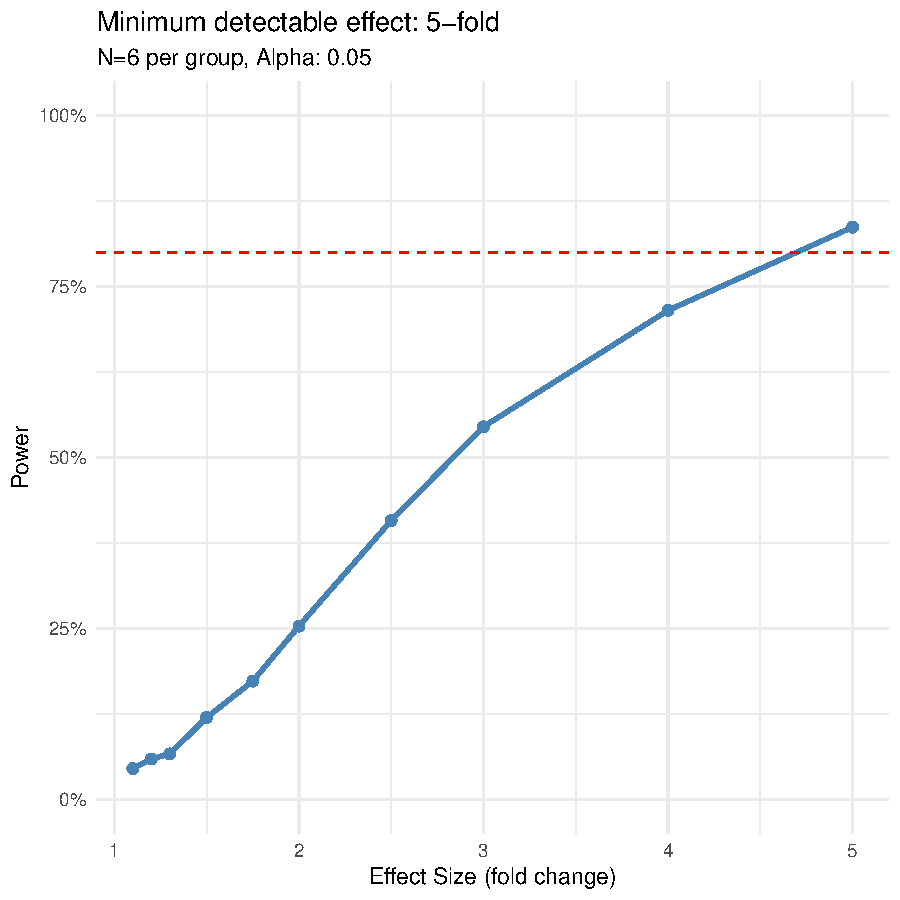
\includegraphics[width=0.7\textwidth]{jss-article-effect-size-plot}
\caption{Power as a function of effect size for fixed sample size (N=6 per group). The minimum detectable effect size represents the smallest fold-change reliably detectable with 80\% power.}
\label{fig:aggregate-effect-curve}
\end{figure}

As shown in Figure~\ref{fig:aggregate-effect-curve}, the analysis indicates that 6 samples per group can reliably detect fold-changes of 5.0 or greater with 80\% power, but smaller effects would require larger sample sizes for adequate detection probability.

\subsubsection{Parameter Sensitivity Analysis}

Aggregate mode facilitates sensitivity analysis by varying distributional assumptions. Different shape parameters reflect varying degrees of heterogeneity and skewness in abundance distributions.

\begin{CodeChunk}
\begin{CodeInput}
R> set.seed(123)
R>
R> # Conservative (high variance) scenario
R> conservative <- power_analysis(
+   "gamma",
+   params = list(shape = 1.5, rate = 0.05),
+   effect_size = 2,
+   target_power = 0.8,
+   find = "sample_size",
+   n_sim = 500
+ )
R>
R> # Moderate variance scenario
R> moderate <- power_analysis(
+   "gamma",
+   params = list(shape = 2.5, rate = 0.05),
+   effect_size = 2,
+   target_power = 0.8,
+   find = "sample_size",
+   n_sim = 500
+ )
R>
R> # Optimistic (low variance) scenario
R> optimistic <- power_analysis(
+   "gamma",
+   params = list(shape = 4, rate = 0.05),
+   effect_size = 2,
+   target_power = 0.8,
+   find = "sample_size",
+   n_sim = 500
+ )
R>
R> cat("Conservative (shape=1.5): N =", conservative$answer, "per group\n")
R> cat("Moderate (shape=2.5):     N =", moderate$answer, "per group\n")
R> cat("Optimistic (shape=4):     N =", optimistic$answer, "per group\n")
\end{CodeInput}
\begin{CodeOutput}
Conservative (shape=1.5): N = 30 per group
Moderate (shape=2.5):     N = 20 per group
Optimistic (shape=4):     N = 12 per group
\end{CodeOutput}
\end{CodeChunk}

The sensitivity analysis demonstrates how distributional assumptions substantially affect sample size requirements. More skewed distributions (lower shape parameters) require larger sample sizes to achieve equivalent power, reflecting the increased variance associated with heavily skewed abundance patterns. This analysis provides bounds for experimental planning under uncertainty about the true underlying distributions.

\section{Per-Peptide Mode Analysis} \label{sec:perpeptide}

While aggregate mode provides rapid power estimates using specified distribution parameters, per-peptide mode leverages pilot data to capture the full heterogeneity of abundance patterns across the peptidome. This mode fits distributions to individual peptides, accommodating the substantial variation in both central tendencies and variance structures that characterizes phosphoproteomics data.

\subsection{Pilot Data and Distribution Fitting}

Per-peptide analysis requires pilot data structured with peptide identifiers, experimental conditions, and quantified abundances. For demonstration, we generate synthetic pilot data representing a heterogeneous peptidome with varying distributional properties across peptides.

\begin{Schunk}
\begin{Sinput}
R> set.seed(42)
R> # Generate heterogeneous pilot data
R> n_peptides <- 100
R> n_per_group <- 4
R> peptide_params <- tibble::tibble(
+    peptide_id = paste0("pep_", sprintf("%04d", 1:n_peptides)),
+    shape = runif(n_peptides, 1.5, 5),
+    rate = runif(n_peptides, 0.01, 0.1)
+  )
R> pilot_data <- peptide_params |>
+    dplyr::rowwise() |>
+    dplyr::mutate(
+      data = list(tibble::tibble(
+        condition = rep(c("control", "treatment"), each = n_per_group),
+        replicate = rep(1:n_per_group, 2),
+        abundance = rgamma(n_per_group * 2, shape = shape, rate = rate)
+      ))
+    ) |>
+    dplyr::ungroup() |>
+    dplyr::select(peptide_id, data) |>
+    tidyr::unnest(data)
\end{Sinput}
\end{Schunk}

The synthetic dataset represents 100 peptides with gamma-distributed abundances, where shape parameters range from 1.5 to 5 and rate parameters from 0.01 to 0.1. This parameterization generates substantial heterogeneity in both mean abundances and variance structures across peptides, reflecting the diversity observed in real phosphoproteomics experiments.

The \fct{fit\_distributions} function fits multiple candidate distributions to each peptide independently, selecting the best-fitting model using AIC-based criteria. For proteomics abundance data, we specify \code{distributions = "continuous"} to evaluate gamma, lognormal, normal, and inverse Gaussian distributions.

\begin{Schunk}
\begin{Sinput}
R> fits <- fit_distributions(
+    pilot_data,
+    id = "peptide_id",
+    group = "condition",
+    value = "abundance",
+    distributions = "continuous"
+  )
R> print(fits)
\end{Sinput}
\begin{Soutput}
peppwr_fits object
------------------
200 peptides fitted

Best fit distribution counts:
  Gamma: 13
  Normal: 22
  Pareto: 124
  Skew Normal: 41
\end{Soutput}
\end{Schunk}

The fitting procedure evaluates each candidate distribution for every peptide, storing fitted parameters, log-likelihood values, and AIC scores. Distribution selection occurs independently for each peptide, accommodating the heterogeneous abundance patterns across the peptidome.

The distribution fitting results reveal substantial heterogeneity across peptides. While the true underlying distributions are gamma (by construction), the fitting process may select alternative distributions for individual peptides due to the limited sample size per peptide (n=4 per group).

\begin{Schunk}
\begin{Sinput}
R> summary(fits)
\end{Sinput}
\begin{Soutput}
Summary of peppwr_fits
======================

Peptides fitted: 200
Failed fits: 0 (0.0%)

Best distribution counts:
  Gamma: 13
  Normal: 22
  Pareto: 124
  Skew Normal: 41

Fit statistics:
  AIC range: [17.6, Inf]
  AIC median: 40.5
  LogLik range: [-Inf, -5.9]
  LogLik median: -18.1
\end{Soutput}
\end{Schunk}

This uncertainty in distribution selection with small sample sizes is expected and does not compromise power analysis validity. The fitted parameters capture the essential statistical properties required for simulation, regardless of the specific distribution family selected. In practice, samples of n$\\geq$15 per group provide more reliable distribution family identification, though the fitted parameters remain useful for power simulation even with smaller pilot datasets.

\subsection{Per-Peptide Power Analysis}

Per-peptide power analysis utilizes the fitted distributions to estimate power across the heterogeneous peptidome. Unlike aggregate mode, which assumes uniform distributional properties, per-peptide analysis accounts for the substantial variation in statistical properties observed across individual peptides.

\begin{Schunk}
\begin{Sinput}
R> set.seed(123)
R> result_pp <- power_analysis(
+    fits,
+    effect_size = 2,
+    n_per_group = 6,
+    find = "power",
+    n_sim = 500
+  )
R> print(result_pp)
\end{Sinput}
\begin{Soutput}
peppwr_power analysis
---------------------
Mode: per_peptide

Power: 55%
Sample size: 6 per group
Effect size: 2.00-fold

Statistical test: wilcoxon
Significance level: 0.05
\end{Soutput}
\end{Schunk}

The analysis reveals substantial heterogeneity in statistical power across the peptidome. Individual peptides exhibit power estimates ranging from near zero to approaching unity, reflecting the different fitted distribution parameters across peptides. The median power across peptides provides a representative estimate for the experiment as a whole.

\begin{Schunk}
\begin{Sinput}
R> plot(result_pp)
\end{Sinput}
\end{Schunk}

\begin{figure}[ht]
\centering
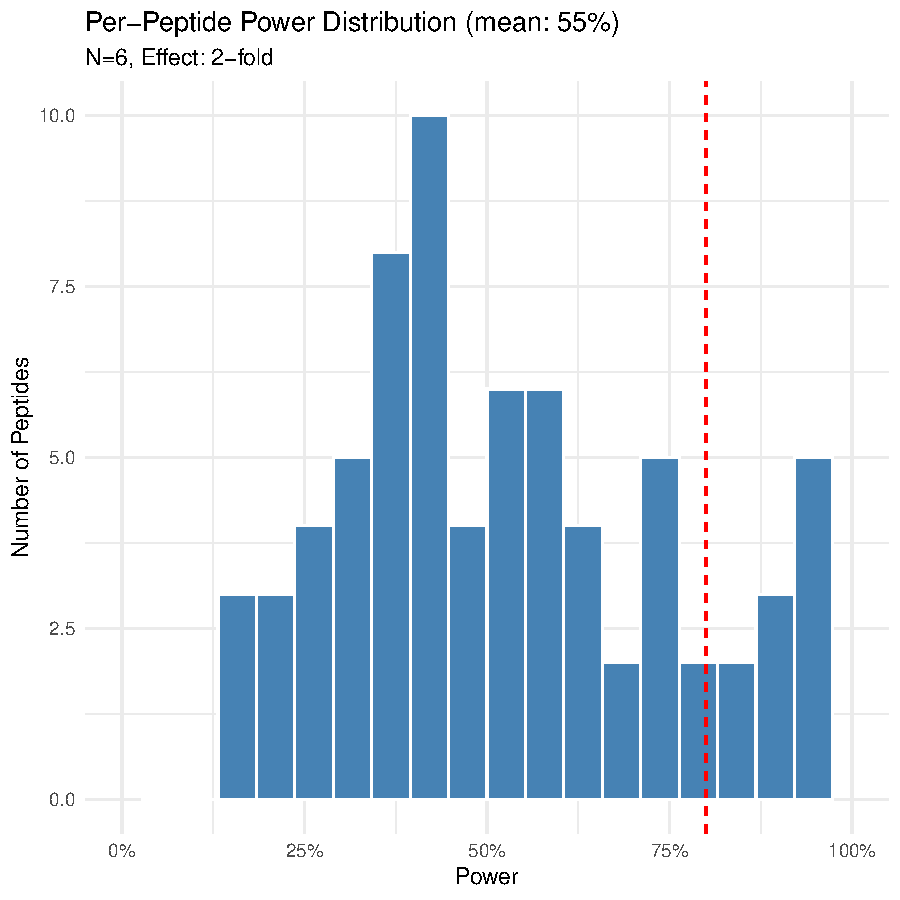
\includegraphics[width=0.7\textwidth]{jss-article-per-peptide-power-plot}
\caption{Distribution of statistical power across peptides for fixed experimental design (N=6 per group, 2-fold effect size). The histogram demonstrates substantial heterogeneity in power estimates, with some peptides achieving near-complete power while others remain substantially underpowered.}
\label{fig:per-peptide-power}
\end{figure}

Figure~\ref{fig:per-peptide-power} illustrates the fundamental advantage of per-peptide analysis: quantifying the expected distribution of power across the heterogeneous peptidome. This visualization enables researchers to understand what fraction of peptides will be adequately powered under specific experimental conditions.

Per-peptide sample size determination addresses the question: "What sample size ensures adequate power for the majority of peptides?" The analysis identifies sample sizes where a specified proportion of peptides achieve target power thresholds.

\begin{Schunk}
\begin{Sinput}
R> set.seed(123)
R> result_n <- power_analysis(
+    fits,
+    effect_size = 2,
+    target_power = 0.8,
+    find = "sample_size",
+    n_sim = 500
+  )
R> print(result_n)
\end{Sinput}
\begin{Soutput}
peppwr_power analysis
---------------------
Mode: per_peptide

Recommended sample size: N=12 per group
Target power: 80%
Effect size: 2.00-fold

Statistical test: wilcoxon
Significance level: 0.05
\end{Soutput}
\end{Schunk}

The recommended sample size represents the point where 50\% of peptides achieve the target power threshold. We use a majority rule where recommended sample sizes target powering most of the peptides, acknowledging that some peptides may remain underpowered at practical sample sizes.

\begin{Schunk}
\begin{Sinput}
R> plot(result_n)
\end{Sinput}
\end{Schunk}

\begin{figure}[ht]
\centering
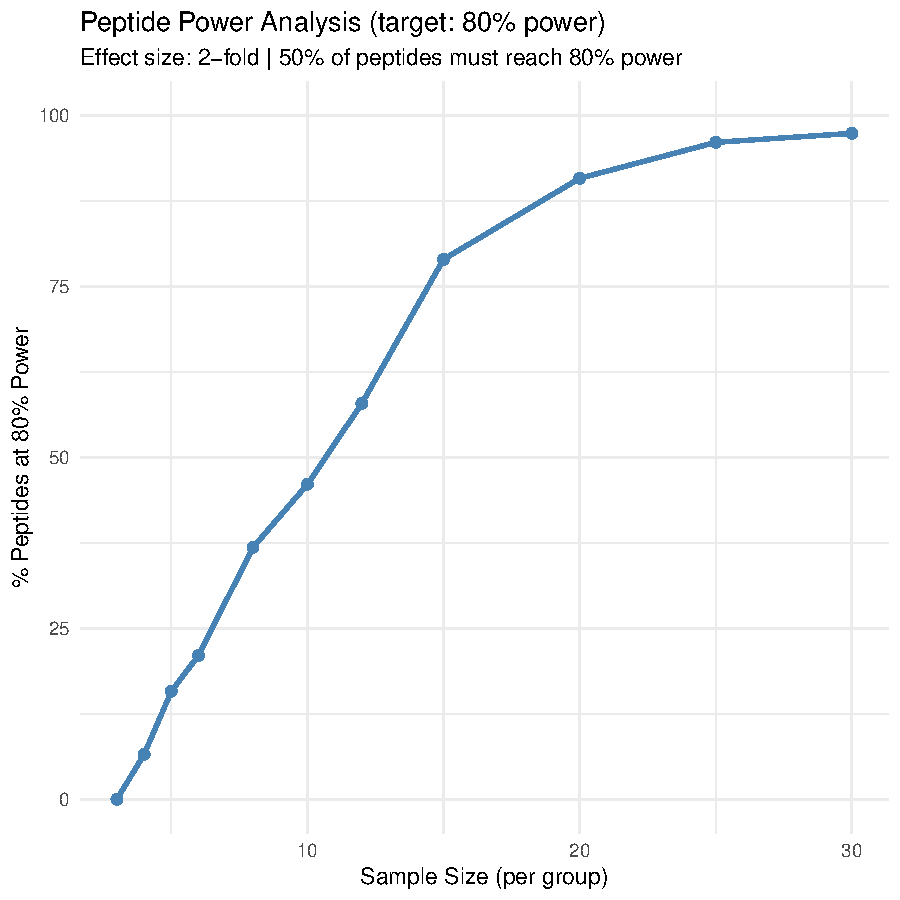
\includegraphics[width=0.7\textwidth]{jss-article-per-peptide-sample-size-plot}
\caption{Peptide threshold curve showing the proportion of peptides achieving 80\% power as a function of sample size. The recommended sample size corresponds to the point where 50\% of peptides achieve target power, representing a practical balance for heterogeneous peptidomes.}
\label{fig:peptide-threshold}
\end{figure}

Figure~\ref{fig:peptide-threshold} presents the peptide threshold curve, a fundamental visualization for per-peptide power analysis. The curve demonstrates how the proportion of well-powered peptides increases with sample size, providing intuitive guidance for experimental design decisions.

Per-peptide analysis provides several key insights for experimental design. First, power varies substantially across peptides due to different underlying abundance distributions and variance structures. Second, we use a majority rule approach where recommended sample sizes target powering most ($\\geq$50\%) of peptides, acknowledging that some peptides may remain underpowered at practical sample sizes. Finally, the analysis enables informed decisions about experimental scope, identifying whether additional samples would meaningfully improve detection rates across the peptidome.

This framework provides realistic power expectations that account for the inherent heterogeneity of phosphoproteomics data, enabling more informed experimental design decisions than aggregate approaches that assume uniform statistical properties across all peptides.

\section*{Acknowledgments}

\begin{leftbar}
All acknowledgments (note the AE spelling) should be collected in this
unnumbered section before the references. It may contain the usual information
about funding and feedback from colleagues/reviewers/etc. Furthermore,
information such as relative contributions of the authors may be added here
(if any).
\end{leftbar}


%% -- Bibliography -------------------------------------------------------------
%% - References need to be provided in a .bib BibTeX database.
%% - All references should be made with \cite, \citet, \citep, \citealp etc.
%%   (and never hard-coded). See the FAQ for details.
%% - JSS-specific markup (\proglang, \pkg, \code) should be used in the .bib.
%% - Titles in the .bib should be in title case.
%% - DOIs should be included where available.

\bibliography{references}


%% -- Appendix (if any) --------------------------------------------------------
%% - After the bibliography with page break.
%% - With proper section titles and _not_ just "Appendix".

\newpage

\begin{appendix}

\section{More technical details} \label{app:technical}

\begin{leftbar}
Appendices can be included after the bibliography (with a page break). Each
section within the appendix should have a proper section title (rather than
just \emph{Appendix}).

For more technical style details, please check out JSS's style FAQ at
\url{https://www.jstatsoft.org/pages/view/style#frequently-asked-questions}
which includes the following topics:
\begin{itemize}
  \item Title vs.\ sentence case.
  \item Graphics formatting.
  \item Naming conventions.
  \item Turning JSS manuscripts into \proglang{R} package vignettes.
  \item Trouble shooting.
  \item Many other potentially helpful details\dots
\end{itemize}
\end{leftbar}


\section[Using BibTeX]{Using \textsc{Bib}{\TeX}} \label{app:bibtex}

\begin{leftbar}
References need to be provided in a \textsc{Bib}{\TeX} file (\code{.bib}). All
references should be made with \verb|\cite|, \verb|\citet|, \verb|\citep|,
\verb|\citealp| etc.\ (and never hard-coded). This commands yield different
formats of author-year citations and allow to include additional details (e.g.,
pages, chapters, \dots) in brackets. In case you are not familiar with these
commands see the JSS style FAQ for details.

Cleaning up \textsc{Bib}{\TeX} files is a somewhat tedious task -- especially
when acquiring the entries automatically from mixed online sources. However,
it is important that informations are complete and presented in a consistent
style to avoid confusions. JSS requires the following format.
\begin{itemize}
  \item JSS-specific markup (\verb|\proglang|, \verb|\pkg|, \verb|\code|) should
    be used in the references.
  \item Titles should be in title case.
  \item Journal titles should not be abbreviated and in title case.
  \item DOIs should be included where available.
  \item Software should be properly cited as well. For \proglang{R} packages
    \code{citation("pkgname")} typically provides a good starting point.
\end{itemize}
\end{leftbar}

\end{appendix}

%% -----------------------------------------------------------------------------


\end{document}
